\chapter{Inductors and RLC Circuits}
\begin{figure}
  \centering
  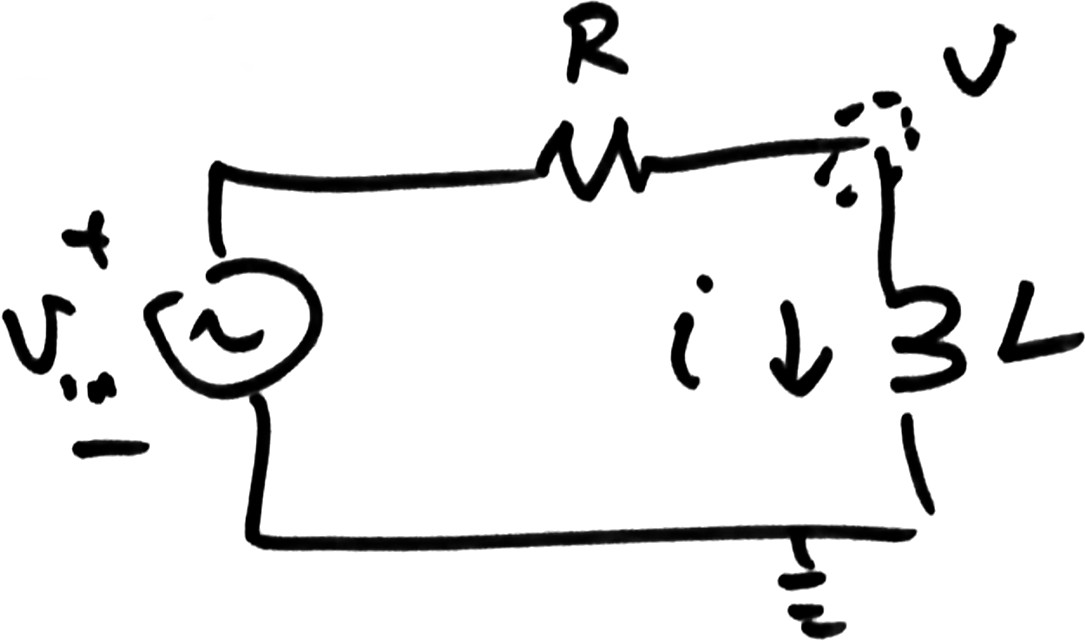
\includegraphics[width=0.4\linewidth]{figures/7/RL-circuit}
  \caption{An RL circuit with an (AC) voltage source.}
  \label{figure:lec7-RL-circuit}
\end{figure}

\section{LR}

The RL circuit in \autoref{figure:lec7-RL-circuit} can be described by the following differential equation:
\begin{align}
  \dod{}{t} i
  &= -\frac{R}{L} i + \frac{1}{L} v_\text{in}.
\end{align}
It has eigenvalue \(\lambda = -\frac{R}{L}\) and time constant \(\tau = \frac{L}{R}\).
Inductance is a ratio of magnetic flux (volt-seconds) to current (amps), so inductance divided by resistance works out to units of seconds.


\section{LC}
\begin{figure}
  \centering
  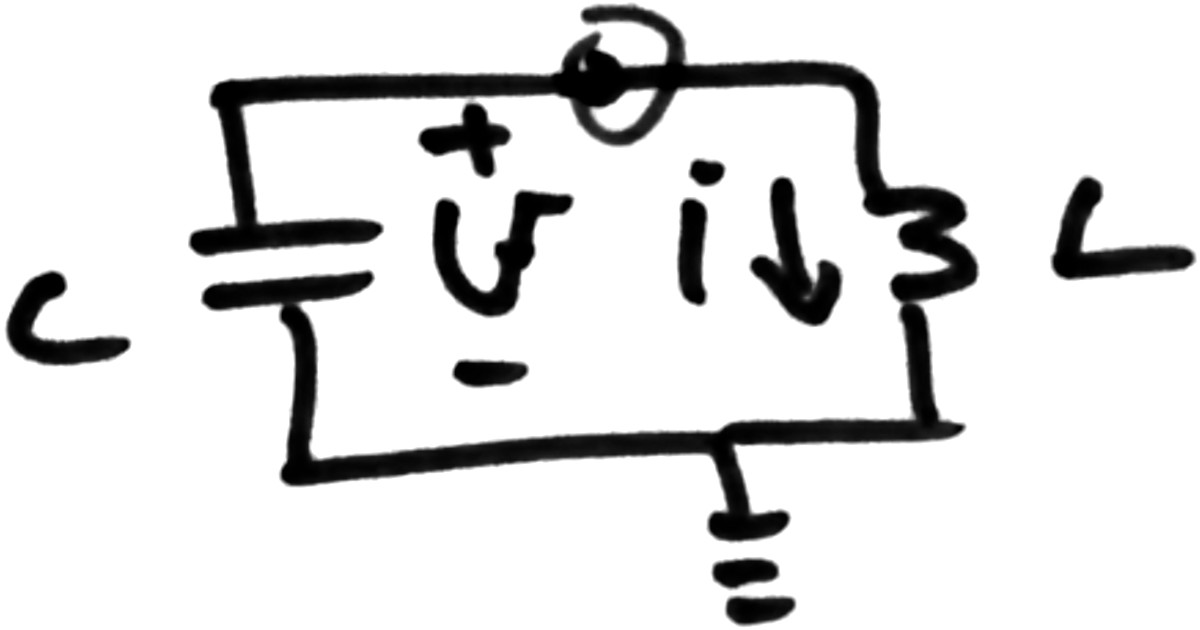
\includegraphics[width=0.4\linewidth]{figures/7/LC-circuit}
  \caption{An LC circuit.}
  \label{figure:lec7-LC-circuit}
\end{figure}
The LC circuit in \autoref{figure:lec7-LC-circuit} can be described by the following two differential equations, which originate in Kirchoff's voltage and current laws, respectively.
\begin{align}
  C \dod{}{t}v + i &= 0\\
  L \dod{}{t}i &= v\\
\intertext{In vector form, with \(\vec x = \begin{bmatrix}
  v \\ i
\end{bmatrix}\),}
  \dod{}{t} \vec x
  &= \begin{bmatrix}
    0 & -\frac{1}{C} \\
    \frac{1}{L} & 0
  \end{bmatrix}
  \vec x
\intertext{This equation can be solved given an initial condition (knowing the value \(\vec x(t_0)\) at some particular time \(t_0\)), yielding a solution for \(v\) and \(i\) that is good at every point in time.
Substituting \(L = 1\unit{H}\) and \(C = 1\unit{F}\),}
  \dod{}{t} \vec x
  &= \begin{bmatrix}
    0 & -1 \\
    1 & 0
  \end{bmatrix}
  \vec x
\intertext{We will analyze this system by taking eigenvalues and eigenvectors of the matrix \(A= \begin{bmatrix}
  0 & -1 \\
  1 & 0
\end{bmatrix}\).
Its eigenvalues are the roots of its characteristic polynomial \(\det\del{\lambda I - A}= \lambda^2 + 1\), which are \(\pm j\).
Call them \(\lambda_1 = j\) and \(\lambda_2 = -j\).
Solving for eigenvectors,}
\lambda_1 \rightsquigarrow
\begin{bmatrix}
  j & 1 \\
-1 & j
\end{bmatrix} \vec v_1 &= \vec 0 \implies \vec v_1 = \begin{bmatrix}
  1 \\ -j
\end{bmatrix} \\
\lambda_2 \rightsquigarrow
\begin{bmatrix}
  -j & 1 \\
-1 & -j
\end{bmatrix} \vec v_2 &= \vec 0 \implies \vec v_2 = \begin{bmatrix}
  1 \\ j
\end{bmatrix}
\end{align}

\subsection{Conjugate pairs}
Notice that \(\lambda_2 = \conj \lambda_1\) and \(\vec v_2 = \conj{\vec v_1}\).
The eigenvalues and eigenvectors come in conjugate pairs because \(A\) is real, and the characteristic polynomial \(p(\lambda) = \det\del{\lambda I - A}\) has real-valued coefficients.
The Fundamental Theorem of Algebra states that a polynomial of degree \(n\) has \(n\) roots.
When the polynomial has real coefficients, then roots are real or occur in complex conjugate pairs:
let \(p(\lambda) = 0\).
Then \(\conj{p(\lambda)} = \conj{0} = 0\):
\begin{align}
  \conj{p(\lambda)}
  &= \conj{\lambda^n} + \conj{a_{n-1} \lambda^{n-1}} + \ldots + a_1 \conj{\lambda} + a_0 =0\\
  &= \del{\conj{\lambda}}^n + a_{n-1} \del{\conj{\lambda}}^{n-1}
+ \ldots + a_1 \conj{\lambda} + a_0 =0
\end{align}
From this we can see that whenver \(\lambda_1\) is a root of the real polynomial \(p(\lambda)\), so is \(\conj{\lambda}_1\).

Conjugate pairing also happens with eigenvectors when \(A\) is real.
If \(A \vec v_1 = \lambda_1 \vec v_1\), then conjugating both sides, we have
\begin{align}
  \conj{\del{A \vec v_1}}
  &= \conj{\del{\lambda_1 \vec v_1}}\\
  A \conj {\vec v_1}
  &= \conj \lambda_1 \conj{\vec v_1}
\end{align}
This shows that \(\conj{\vec v_1}\) is an eigenvector as well, completing a pair with \(\vec v_1\).

\subsection{Back to LC circuit}
\begin{figure}
  \centering
  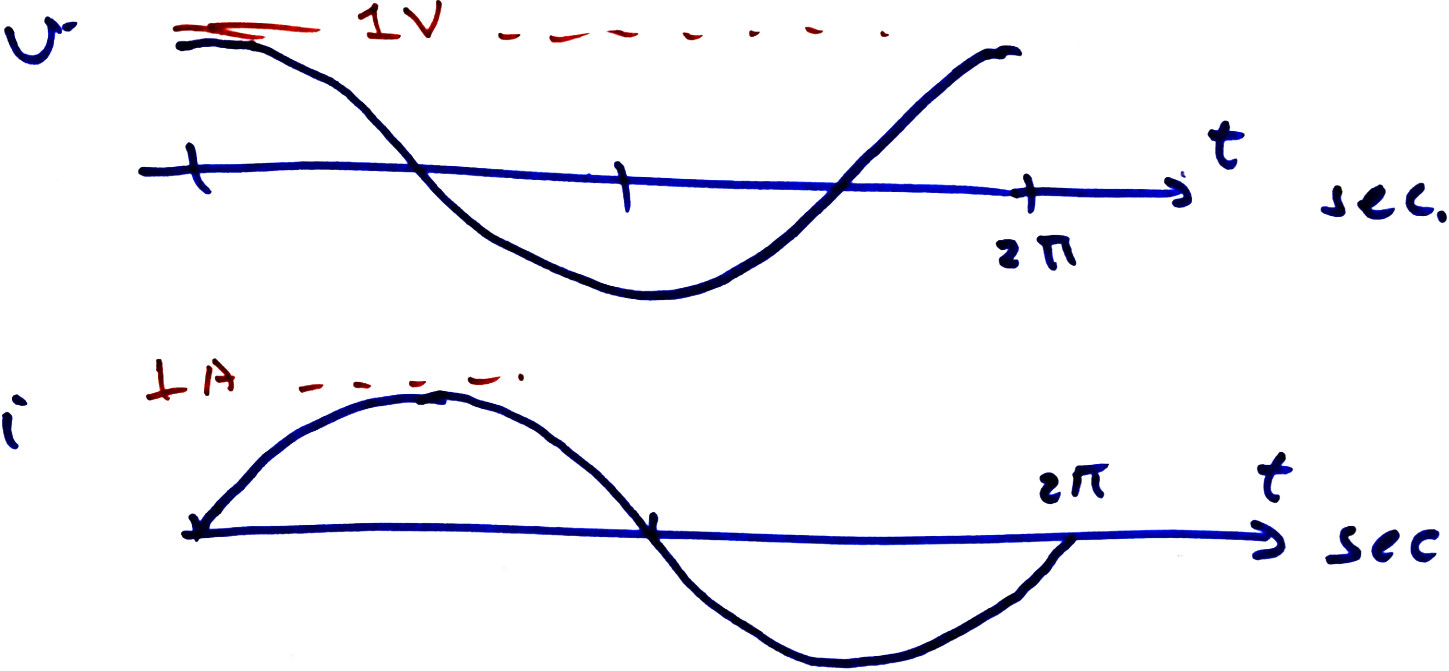
\includegraphics[width=0.6\linewidth]{figures/7/LC-vi}
  \caption{Current and voltage of an oscillating LC circuit.}
  \label{figure:lec7-LC-vi}
\end{figure}
\begin{figure}
  \centering
  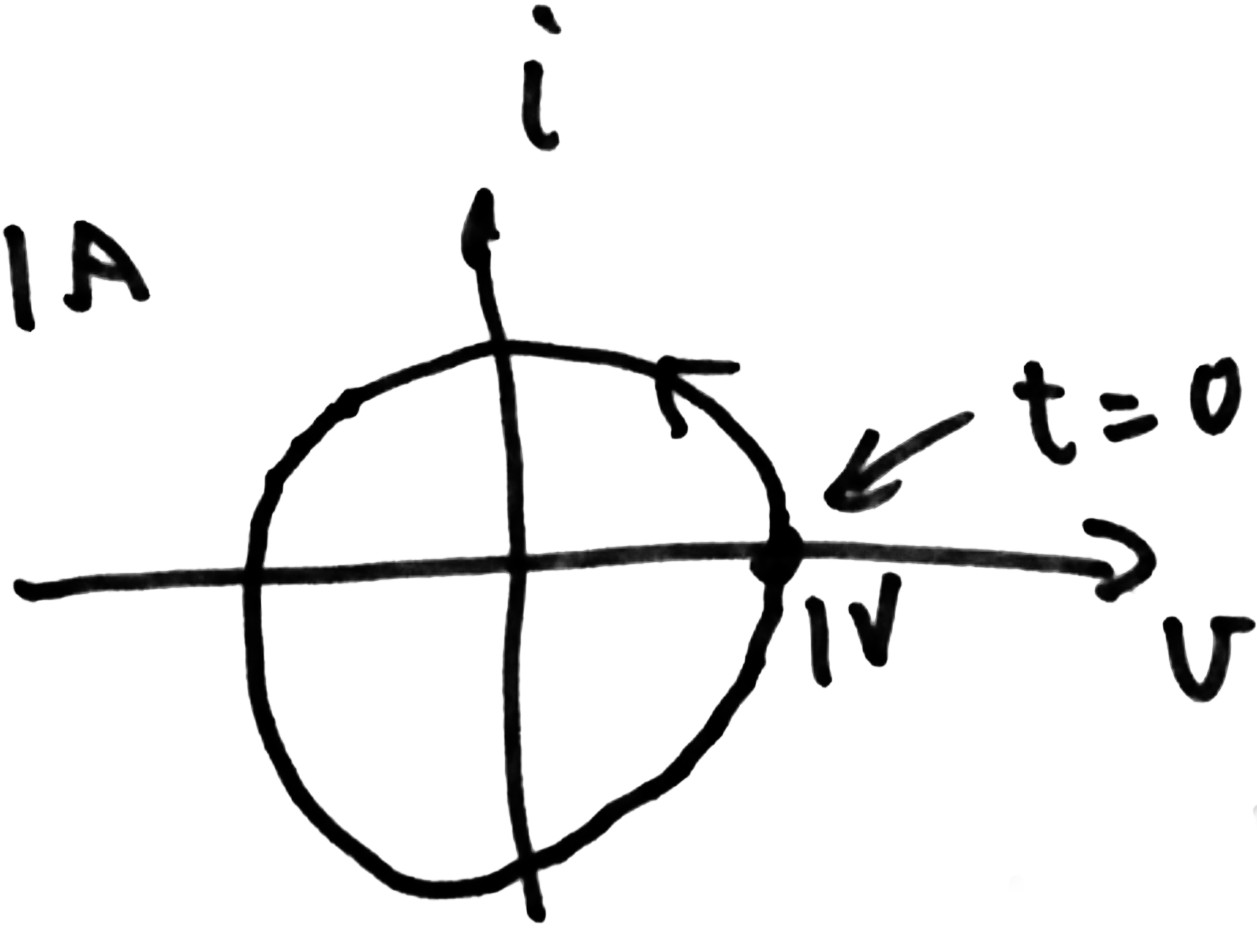
\includegraphics[width=0.3\linewidth]{figures/7/LC-iv-parametric}
  \caption{Phase portrait of an oscillating LC circuit.}
  \label{figure:lec7-iv-parametric}
\end{figure}

Let's take initial condition \(\vec{x}(0) = \begin{bmatrix}
  1\unit{V}\\
  0\unit{A}
\end{bmatrix}\).
As a combination of \(\vec v_1\) and \(\vec v_2\),
\begin{align}
  \vec x(0) &= \frac{1}{2}
  \underbrace{\begin{bmatrix}
    1 \\
    -j
  \end{bmatrix}}_{\vec v_1}
+ \frac{1}{2}
\underbrace{\begin{bmatrix}
  1 \\
  j
\end{bmatrix}}_{\vec v_2}
\intertext{Therefore, the same linear combination will construct \(\vec x(t)\) from its constituent modes.}
\vec x(t)
 &= \frac{1}{2}
\underbrace{\begin{bmatrix}
  1 \\
  -j
\end{bmatrix}}_{\vec v_1}
e^{jt}
+ \frac{1}{2}
\underbrace{\begin{bmatrix}
1 \\
j
\end{bmatrix}}_{\vec v_2}
e^{-jt}\\
&= \begin{bmatrix}
  \frac{1}{2} e^{jt} + \frac{1}{2} e^{-jt}
            \\[3pt] %otherwise a bit tight
\frac{1}{j} e^{jt} - \frac{1}{2j} e^{-jt}
\end{bmatrix}
= \begin{bmatrix}
  \cos t \\
  \sin t
\end{bmatrix},
% \intertext{
% }
\end{align}
which follows from the identities
\(\cos \theta = \frac{1}{2} \del{e^{j\theta} + e^{-j\theta}}\) and
\(\sin \theta = \frac{1}{2j} \del{e^{j\theta} - e^{-j\theta}}\),
which are both consequences of Euler's formula
\(e^{j\theta} = \cos \theta + j\sin \theta\).



Under an oscilloscope, \(v(t) = \sin t\) and \(i(t) = \cos t\) might appear as they do in \autoref{figure:lec7-LC-vi}.
If \(\vec x(t)\) is plotted as a parametric curve in the plane (called a \emph{phase portrait}), the result is a counterclockwise traversal of the unit circle, shown in \autoref{figure:lec7-iv-parametric}.
This means that the \(\vec x\) vector has constant length:
\begin{align}
  v^2 + i^2 &= 1 \ \text{for all \(t\).}
\end{align}

\subsection{Euler's formula}
Euler's formula states that \(e^{j\theta} = \cos \theta + j\sin \theta\).
This can be derived from the series expansion of the exponential function around \(\theta=0\),
\begin{align}
  e^z &= 1 + z + \frac{1}{2!} z^2 + \ldots
  \intertext{Substituting \(z = j\theta\), we have}
e^{j\theta}
  &= 1 + j\theta + \frac{-1}{2!} \theta^2 +  \frac{-j}{3!} \theta^3 + \ldots,
  \intertext{whose even terms add to \(\cos{\theta}\):}
  \cos{\theta}
  &= 1 - \frac{1}{2!} \theta^2 + \frac{1}{4!} \theta^4 + \ldots,
\intertext{and whose odd terms add to \(j\sin \theta\):}
  \sin{\theta}
  &= \theta - \frac{1}{3!} \theta^3 + \frac{1}{5!} \theta^5 \ldots.
\end{align}

\section{LRC}
\begin{figure}
  \centering
  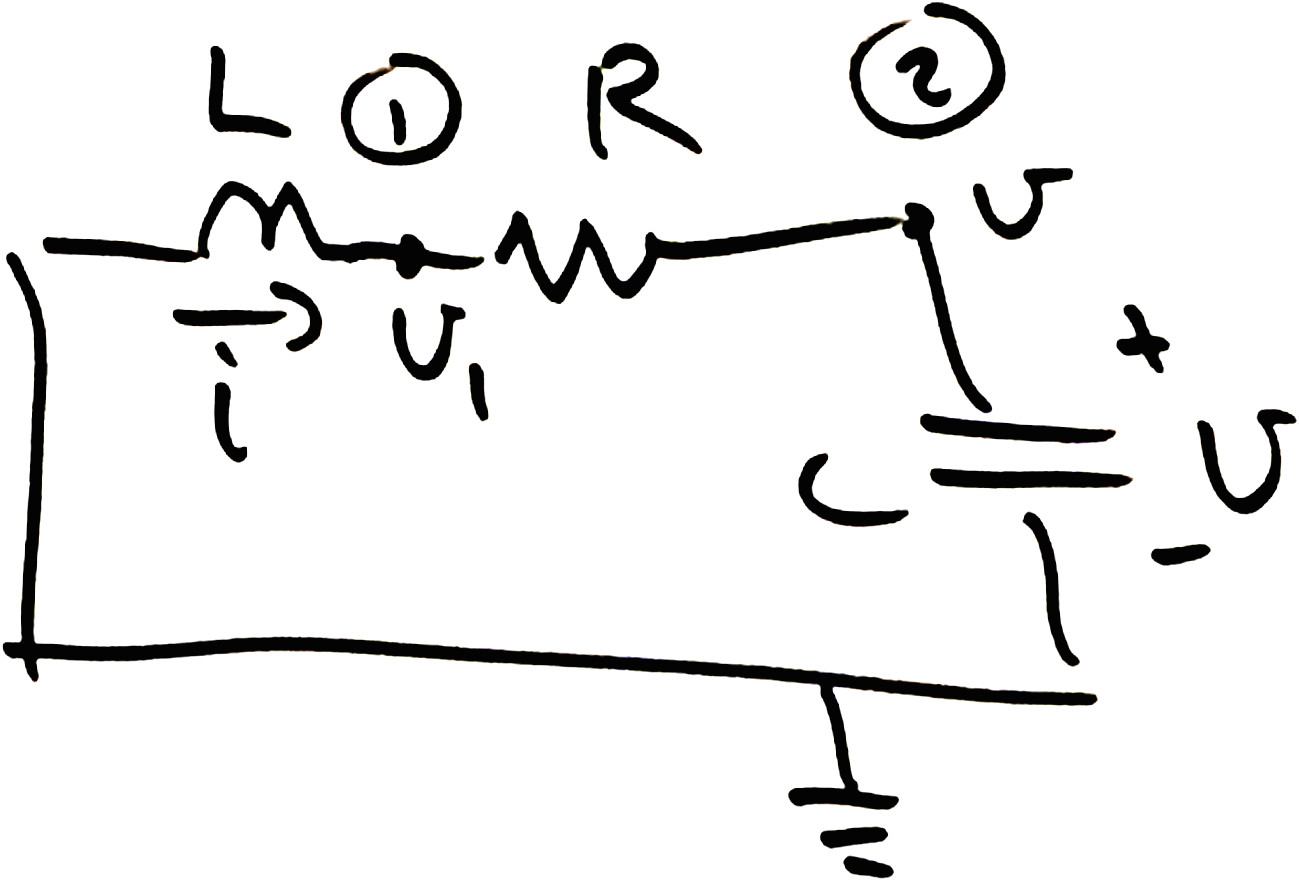
\includegraphics[width=0.5\linewidth]{figures/7/LRC-circuit}
  \caption{An LRC circuit.}
  \label{figure:lec7-LRC-circuit}
\end{figure}
\begin{figure}
  \centering
  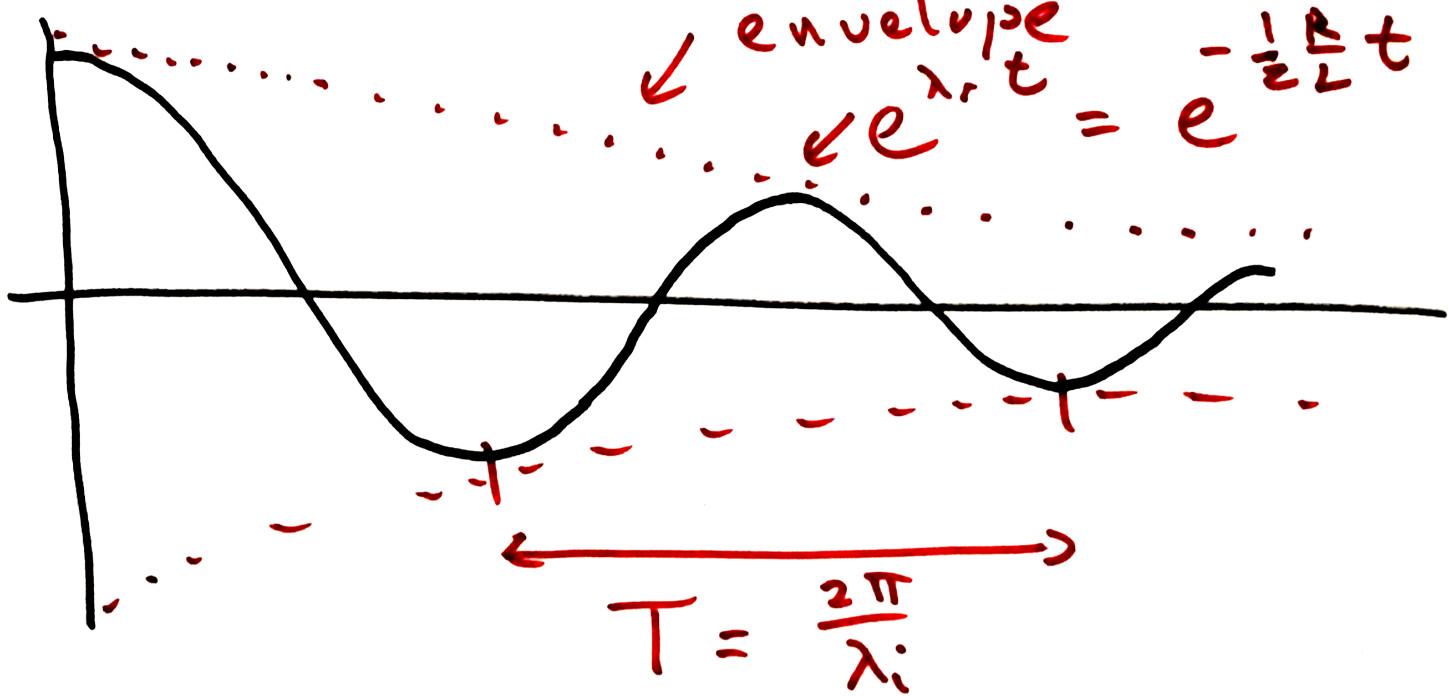
\includegraphics[width=0.8\linewidth]{figures/7/decaying-exponential}
  \caption{The effects of the real and imaginary parts of an eigenvalue \(\lambda = \lambda_r + j\lambda_i\), when neither is zero.}
  \label{figure:lec7-decaying-exponential}
\end{figure}
The following node equations describe the LRC circuit in \autoref{figure:lec7-LRC-circuit}:
\begin{alignat}{3}
  & (1) \quad & -i + \frac{v_1 - v}{R} & = 0\label{eq:lec7-KCL}\\
  & (2) \quad & \frac{v - v_1}{R} + C \dod{}{t} v &= 0\\
  & (3) \quad & L \dod{}{t}i &= -v_1
\end{alignat}
After using \autoref{eq:lec7-KCL} to eliminate \(v_1\), we have the following two differential equations:
\begin{align}
  C \dod{}{t} v &= i \\
  L \dod{}{t} i &= -Ri - v
\intertext{or, in vector form,}
  \dod{}{t} \begin{bmatrix}
    v\\i
  \end{bmatrix}
  &= \begin{bmatrix}
    0 & \frac{1}{C} \\[3pt]
    -\frac{1}{L} & -\frac{R}{L}
  \end{bmatrix}
  \begin{bmatrix}
    v \\ i
  \end{bmatrix}
  \label{eq:lec7-lrc-A}
\intertext{From its characteristic equation}
  0 &= \lambda^2 + \frac{R}{L} \lambda + \frac{1}{LC},
\intertext{we obtain eigenvalues}
  \lambda_{1,2}
  &= -\frac{1}{2} \frac{R}{L} \pm j\sqrt{\del{\frac{1}{2}\frac{R}{L}}^2 - \frac{1}{LC}}.
\end{align}

As \(R\) increases from zero, the eigenvalues move in significant ways.
\begin{enumerate}
  \item When \(R = 0\), the eigenvalues are the imaginary pair \(\pm j\sqrt{\frac{1}{LC}}\).
  \item When \(\del{\frac{1}{2}\frac{R}{L}}^2=- \frac{1}{LC}\), the eigenvalues are both \(-\frac{1}{2}\frac{R}{L}\).
  \item When \(\del{\frac{1}{2}\frac{R}{L}}^2 > - \frac{1}{LC}\), the eigenvalues are distinct and real-valued.
\end{enumerate}
Between (1) and (2), the eigenvalues are neither real nor pure imaginary:
\begin{align}
  \lambda_{1,2}
&= \underbrace{-\frac{1}{2} \frac{R}{L}}_{\lambda_r} \pm j \underbrace{\sqrt{\del{\frac{1}{2}\frac{R}{L}}^2 - \frac{1}{LC}}}_{\lambda_i} = \lambda_r \pm j\lambda_i
  \intertext{The time domain response will incorporate \(e^{\lambda t}\), which has the following trigonometric interpretation:}
  e^{\del{\lambda_r + j\lambda_i} t}
  &= e^{\lambda_r t} e^{j\lambda_i t} \\
  &= e^{\lambda_r t} \del{\cos \lambda_i t + j\sin \lambda_i t},
\end{align}
a sinusoid of angular frequency \(\lambda_i\) under an envelope with rate \(\lambda_r\), as shown in \autoref{figure:lec7-decaying-exponential}.
